\begin{frame}
    \frametitle{Breakdown of Results}
    4 transition scenarios sought to minimize undersupply and under capacity of 
        all commodities.
    \begin{enumerate}
            \item EG01-23 ($P(t) = P_0$)
        \item EG01-24 ($P(t) = P_0 + rt$)
        \item EG01-29 ($P(t) = P_0)$
        \item EG01-30 ($P(t) = P_0 + rt$)
    \end{enumerate}

This is achieved by:
\begin{enumerate}
    \item Comparison of prediction methods for each of 4 scenarios is conducted 
    to determine the best method. 
    \item Sensitivity analysis of power supply buffer is conducted to determine 
    best buffer size. 
    \item Using best prediction method, look ahead rate, buffer size, demonstrate \deploy 
    deploying reactor and supporting facilities to meet power demand 
    for 4 scenarios. 
\end{enumerate}

\end{frame}


\begin{frame}
        \frametitle{EG01 - EG23}

\begin{figure}[H]
	\centering
	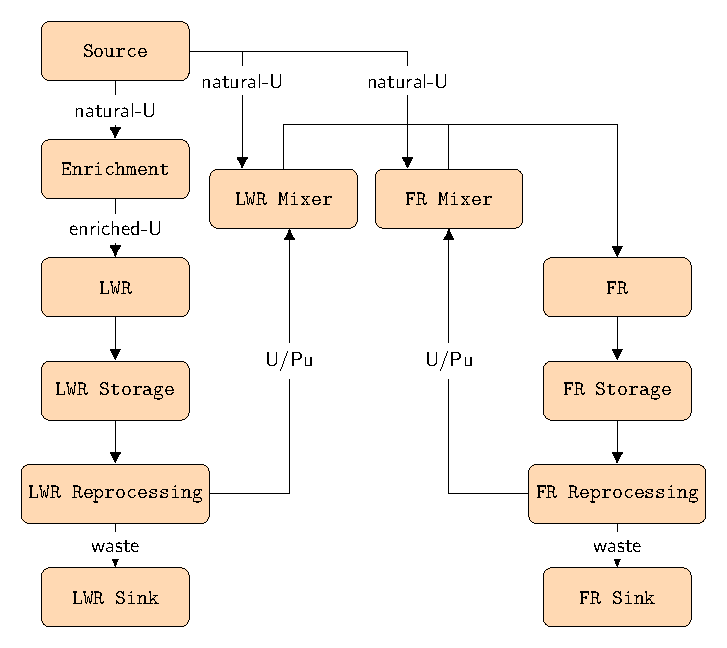
\includegraphics[width=\textwidth]{images/23flow.pdf}
	\hfill
	\caption{EG01-EG23 fuel cycle as modeled in \cyclus.}
	\label{fig:23flow}
\end{figure}
\end{frame}





\begin{frame}
        \frametitle{EG01 - EG23}

\begin{figure}[H]
	\centering
	\includegraphics[width=\textwidth]{images/30flow.pdf}
	\hfill
	\caption{EG01-EG30.}
	\label{fig:30flow}
\end{figure}

